% Options for packages loaded elsewhere
\PassOptionsToPackage{unicode}{hyperref}
\PassOptionsToPackage{hyphens}{url}
%
\documentclass[
]{article}
\usepackage{lmodern}
\usepackage{amssymb,amsmath}
\usepackage{ifxetex,ifluatex}
\ifnum 0\ifxetex 1\fi\ifluatex 1\fi=0 % if pdftex
  \usepackage[T1]{fontenc}
  \usepackage[utf8]{inputenc}
  \usepackage{textcomp} % provide euro and other symbols
\else % if luatex or xetex
  \usepackage{unicode-math}
  \defaultfontfeatures{Scale=MatchLowercase}
  \defaultfontfeatures[\rmfamily]{Ligatures=TeX,Scale=1}
\fi
% Use upquote if available, for straight quotes in verbatim environments
\IfFileExists{upquote.sty}{\usepackage{upquote}}{}
\IfFileExists{microtype.sty}{% use microtype if available
  \usepackage[]{microtype}
  \UseMicrotypeSet[protrusion]{basicmath} % disable protrusion for tt fonts
}{}
\makeatletter
\@ifundefined{KOMAClassName}{% if non-KOMA class
  \IfFileExists{parskip.sty}{%
    \usepackage{parskip}
  }{% else
    \setlength{\parindent}{0pt}
    \setlength{\parskip}{6pt plus 2pt minus 1pt}}
}{% if KOMA class
  \KOMAoptions{parskip=half}}
\makeatother
\usepackage{xcolor}
\IfFileExists{xurl.sty}{\usepackage{xurl}}{} % add URL line breaks if available
\IfFileExists{bookmark.sty}{\usepackage{bookmark}}{\usepackage{hyperref}}
\hypersetup{
  pdftitle={Econometrics II - Problem 1},
  pdfauthor={William Radaic Peron},
  hidelinks,
  pdfcreator={LaTeX via pandoc}}
\urlstyle{same} % disable monospaced font for URLs
\usepackage[margin=1in]{geometry}
\usepackage{color}
\usepackage{fancyvrb}
\newcommand{\VerbBar}{|}
\newcommand{\VERB}{\Verb[commandchars=\\\{\}]}
\DefineVerbatimEnvironment{Highlighting}{Verbatim}{commandchars=\\\{\}}
% Add ',fontsize=\small' for more characters per line
\usepackage{framed}
\definecolor{shadecolor}{RGB}{248,248,248}
\newenvironment{Shaded}{\begin{snugshade}}{\end{snugshade}}
\newcommand{\AlertTok}[1]{\textcolor[rgb]{0.94,0.16,0.16}{#1}}
\newcommand{\AnnotationTok}[1]{\textcolor[rgb]{0.56,0.35,0.01}{\textbf{\textit{#1}}}}
\newcommand{\AttributeTok}[1]{\textcolor[rgb]{0.77,0.63,0.00}{#1}}
\newcommand{\BaseNTok}[1]{\textcolor[rgb]{0.00,0.00,0.81}{#1}}
\newcommand{\BuiltInTok}[1]{#1}
\newcommand{\CharTok}[1]{\textcolor[rgb]{0.31,0.60,0.02}{#1}}
\newcommand{\CommentTok}[1]{\textcolor[rgb]{0.56,0.35,0.01}{\textit{#1}}}
\newcommand{\CommentVarTok}[1]{\textcolor[rgb]{0.56,0.35,0.01}{\textbf{\textit{#1}}}}
\newcommand{\ConstantTok}[1]{\textcolor[rgb]{0.00,0.00,0.00}{#1}}
\newcommand{\ControlFlowTok}[1]{\textcolor[rgb]{0.13,0.29,0.53}{\textbf{#1}}}
\newcommand{\DataTypeTok}[1]{\textcolor[rgb]{0.13,0.29,0.53}{#1}}
\newcommand{\DecValTok}[1]{\textcolor[rgb]{0.00,0.00,0.81}{#1}}
\newcommand{\DocumentationTok}[1]{\textcolor[rgb]{0.56,0.35,0.01}{\textbf{\textit{#1}}}}
\newcommand{\ErrorTok}[1]{\textcolor[rgb]{0.64,0.00,0.00}{\textbf{#1}}}
\newcommand{\ExtensionTok}[1]{#1}
\newcommand{\FloatTok}[1]{\textcolor[rgb]{0.00,0.00,0.81}{#1}}
\newcommand{\FunctionTok}[1]{\textcolor[rgb]{0.00,0.00,0.00}{#1}}
\newcommand{\ImportTok}[1]{#1}
\newcommand{\InformationTok}[1]{\textcolor[rgb]{0.56,0.35,0.01}{\textbf{\textit{#1}}}}
\newcommand{\KeywordTok}[1]{\textcolor[rgb]{0.13,0.29,0.53}{\textbf{#1}}}
\newcommand{\NormalTok}[1]{#1}
\newcommand{\OperatorTok}[1]{\textcolor[rgb]{0.81,0.36,0.00}{\textbf{#1}}}
\newcommand{\OtherTok}[1]{\textcolor[rgb]{0.56,0.35,0.01}{#1}}
\newcommand{\PreprocessorTok}[1]{\textcolor[rgb]{0.56,0.35,0.01}{\textit{#1}}}
\newcommand{\RegionMarkerTok}[1]{#1}
\newcommand{\SpecialCharTok}[1]{\textcolor[rgb]{0.00,0.00,0.00}{#1}}
\newcommand{\SpecialStringTok}[1]{\textcolor[rgb]{0.31,0.60,0.02}{#1}}
\newcommand{\StringTok}[1]{\textcolor[rgb]{0.31,0.60,0.02}{#1}}
\newcommand{\VariableTok}[1]{\textcolor[rgb]{0.00,0.00,0.00}{#1}}
\newcommand{\VerbatimStringTok}[1]{\textcolor[rgb]{0.31,0.60,0.02}{#1}}
\newcommand{\WarningTok}[1]{\textcolor[rgb]{0.56,0.35,0.01}{\textbf{\textit{#1}}}}
\usepackage{graphicx,grffile}
\makeatletter
\def\maxwidth{\ifdim\Gin@nat@width>\linewidth\linewidth\else\Gin@nat@width\fi}
\def\maxheight{\ifdim\Gin@nat@height>\textheight\textheight\else\Gin@nat@height\fi}
\makeatother
% Scale images if necessary, so that they will not overflow the page
% margins by default, and it is still possible to overwrite the defaults
% using explicit options in \includegraphics[width, height, ...]{}
\setkeys{Gin}{width=\maxwidth,height=\maxheight,keepaspectratio}
% Set default figure placement to htbp
\makeatletter
\def\fps@figure{htbp}
\makeatother
\setlength{\emergencystretch}{3em} % prevent overfull lines
\providecommand{\tightlist}{%
  \setlength{\itemsep}{0pt}\setlength{\parskip}{0pt}}
\setcounter{secnumdepth}{-\maxdimen} % remove section numbering

\title{Econometrics II - Problem 1}
\author{William Radaic Peron}
\date{\today}

\begin{document}
\maketitle

Loading the database and creating dummy variables:

\begin{Shaded}
\begin{Highlighting}[]
\NormalTok{df <-}\StringTok{ }\KeywordTok{read_excel}\NormalTok{(}\StringTok{"RS_USD.xlsx"}\NormalTok{)}


\KeywordTok{names}\NormalTok{(df)[}\KeywordTok{names}\NormalTok{(df) }\OperatorTok{==}\StringTok{ "R$/US$"}\NormalTok{] <-}\StringTok{ "p"}

\KeywordTok{names}\NormalTok{(df)[}\KeywordTok{names}\NormalTok{(df) }\OperatorTok{==}\StringTok{ "Variação (em %)"}\NormalTok{] <-}\StringTok{ "delta"}

\KeywordTok{names}\NormalTok{(df)[}\KeywordTok{names}\NormalTok{(df) }\OperatorTok{==}\StringTok{ "Data"}\NormalTok{] <-}\StringTok{ "date"}

\NormalTok{sign <-}\StringTok{ }\KeywordTok{as.numeric}\NormalTok{(df}\OperatorTok{$}\NormalTok{delta }\OperatorTok{>}\StringTok{ }\DecValTok{0}\NormalTok{)}

\NormalTok{count <-}\StringTok{ }\KeywordTok{c}\NormalTok{(}\DecValTok{1}\OperatorTok{:}\DecValTok{2153}\NormalTok{)}

\NormalTok{df <-}\StringTok{ }\KeywordTok{data.frame}\NormalTok{(count, df, sign)}
\end{Highlighting}
\end{Shaded}

Before constructing our models, we need to check (intuitively) if the
series at hand is \emph{stationary} and \emph{ergodic}. For this, we're
going to plot the time series, its autocorrelations and partial
autocorrelations.

\begin{Shaded}
\begin{Highlighting}[]
\NormalTok{pplot <-}\StringTok{ }\KeywordTok{ggplot}\NormalTok{(}\DataTypeTok{data =}\NormalTok{ df, }\KeywordTok{aes}\NormalTok{(}\DataTypeTok{x =}\NormalTok{ date, }\DataTypeTok{y =}\NormalTok{ p)) }\OperatorTok{+}\StringTok{ }\KeywordTok{geom_line}\NormalTok{() }\OperatorTok{+}\StringTok{ }
\StringTok{    }\KeywordTok{ggtitle}\NormalTok{(}\StringTok{"USD/BRL, Price"}\NormalTok{) }\OperatorTok{+}\StringTok{ }\KeywordTok{theme_few}\NormalTok{()}
\NormalTok{pplot}
\end{Highlighting}
\end{Shaded}

\begin{center}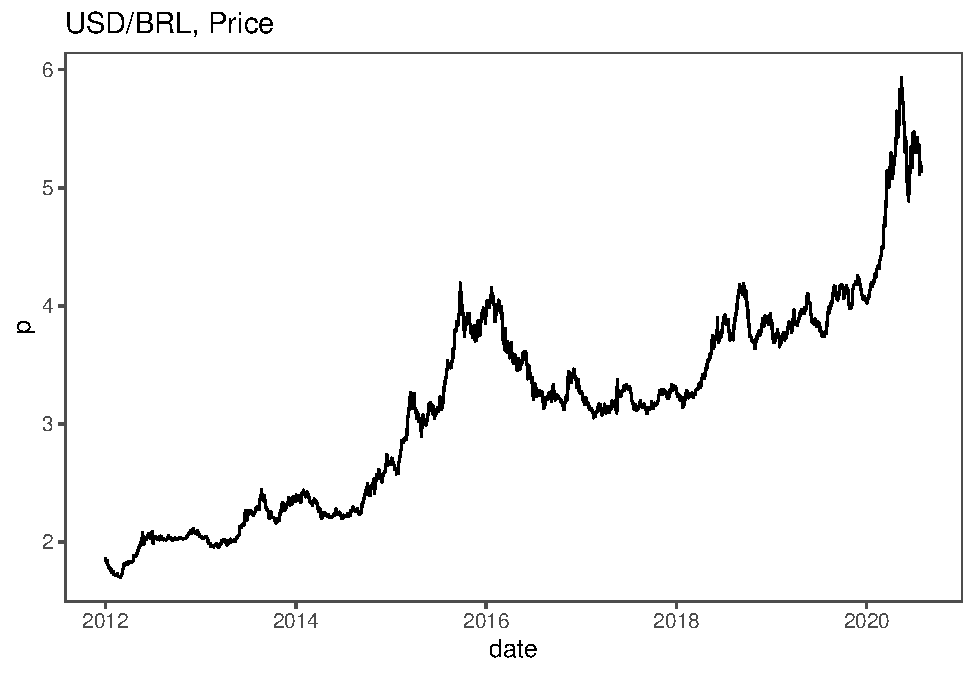
\includegraphics{Econo2_P1_files/figure-latex/plots-1} \end{center}

\begin{Shaded}
\begin{Highlighting}[]
\NormalTok{deltaplot <-}\StringTok{ }\KeywordTok{ggplot}\NormalTok{(}\DataTypeTok{data =}\NormalTok{ df, }\KeywordTok{aes}\NormalTok{(}\DataTypeTok{x =}\NormalTok{ date, }\DataTypeTok{y =}\NormalTok{ delta)) }\OperatorTok{+}\StringTok{ }\KeywordTok{geom_line}\NormalTok{() }\OperatorTok{+}\StringTok{ }
\StringTok{    }\KeywordTok{ggtitle}\NormalTok{(}\StringTok{"USD/BRL, %"}\NormalTok{) }\OperatorTok{+}\StringTok{ }\KeywordTok{theme_few}\NormalTok{()}
\NormalTok{deltaplot}
\end{Highlighting}
\end{Shaded}

\begin{center}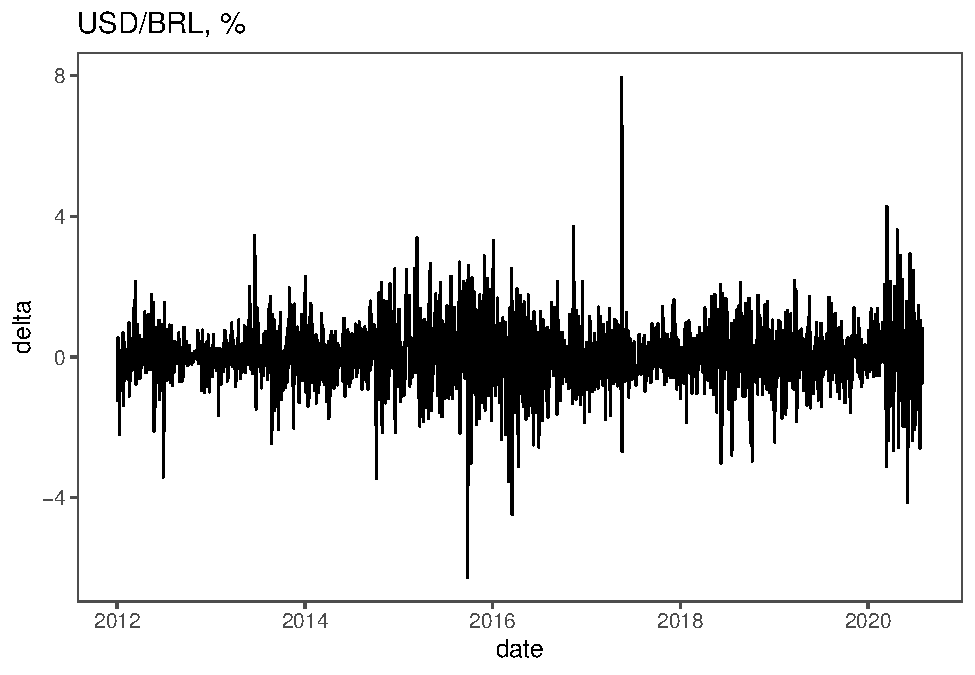
\includegraphics{Econo2_P1_files/figure-latex/plots-2} \end{center}

\begin{Shaded}
\begin{Highlighting}[]
\NormalTok{dummyplot <-}\StringTok{ }\KeywordTok{ggplot}\NormalTok{(}\DataTypeTok{data =}\NormalTok{ df, }\KeywordTok{aes}\NormalTok{(}\DataTypeTok{x =}\NormalTok{ count, }\DataTypeTok{y =}\NormalTok{ sign)) }\OperatorTok{+}\StringTok{ }\KeywordTok{geom_line}\NormalTok{() }\OperatorTok{+}\StringTok{ }
\StringTok{    }\KeywordTok{ggtitle}\NormalTok{(}\StringTok{"USD/BRL, +/-"}\NormalTok{) }\OperatorTok{+}\StringTok{ }\KeywordTok{xlim}\NormalTok{(}\DecValTok{1}\NormalTok{, }\DecValTok{200}\NormalTok{) }\OperatorTok{+}\StringTok{ }\KeywordTok{theme_few}\NormalTok{()}
\NormalTok{dummyplot}
\end{Highlighting}
\end{Shaded}

\begin{verbatim}
## Warning: Removed 1953 row(s) containing missing values (geom_path).
\end{verbatim}

\begin{center}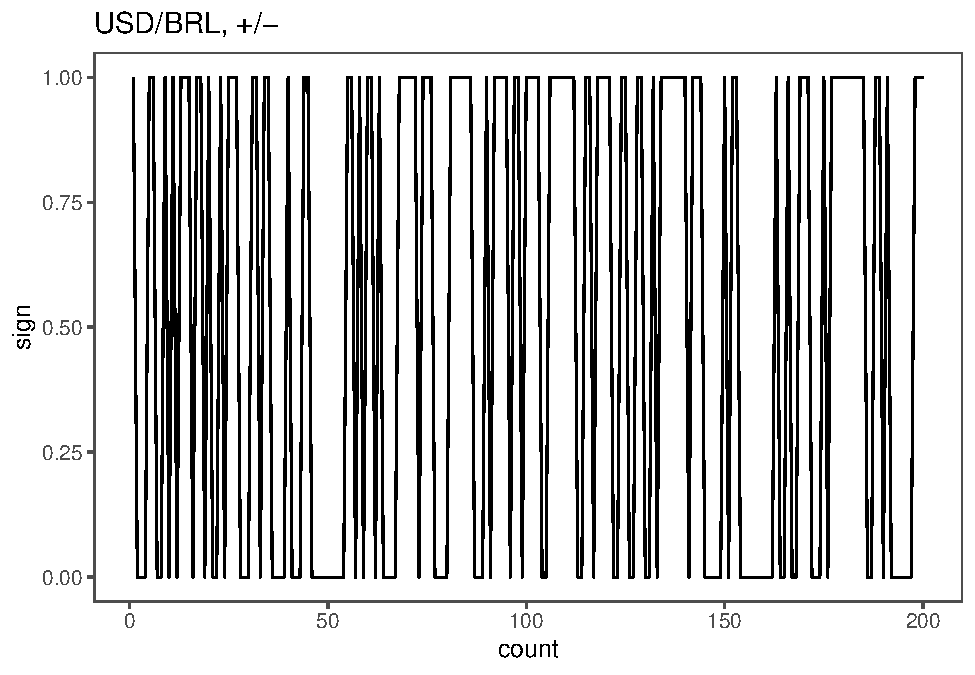
\includegraphics{Econo2_P1_files/figure-latex/plots-3} \end{center}

\begin{Shaded}
\begin{Highlighting}[]
\CommentTok{# For delta}

\NormalTok{acf_delta <-}\StringTok{ }\KeywordTok{Acf}\NormalTok{(df}\OperatorTok{$}\NormalTok{delta, }\DataTypeTok{lag.max =} \DecValTok{5000}\NormalTok{)}
\end{Highlighting}
\end{Shaded}

\begin{center}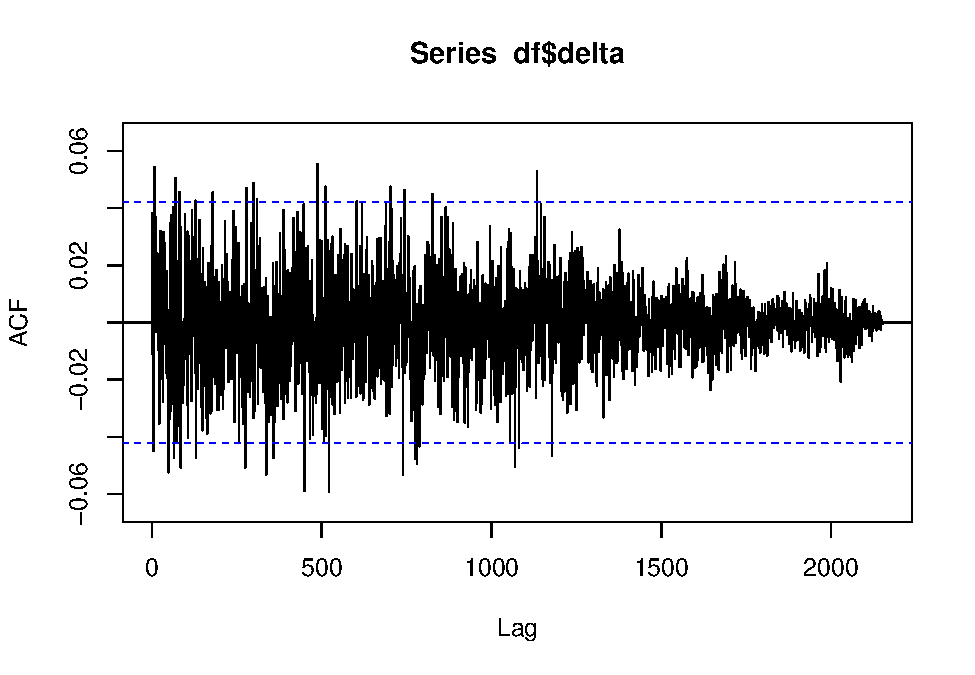
\includegraphics{Econo2_P1_files/figure-latex/plots-4} \end{center}

\begin{Shaded}
\begin{Highlighting}[]
\NormalTok{acf_test_values <-}\StringTok{ }\NormalTok{acf_delta}\OperatorTok{$}\NormalTok{acf}\OperatorTok{/}\KeywordTok{sd}\NormalTok{(acf_delta}\OperatorTok{$}\NormalTok{acf)}

\KeywordTok{head}\NormalTok{(}\KeywordTok{data.frame}\NormalTok{(acf_test_values))}
\end{Highlighting}
\end{Shaded}

\begin{verbatim}
##   acf_test_values
## 1      37.9547672
## 2       1.4506537
## 3      -0.4173129
## 4       0.2125873
## 5      -1.7053782
## 6       0.5358210
\end{verbatim}

\begin{Shaded}
\begin{Highlighting}[]
\NormalTok{facst <-}\StringTok{ }\KeywordTok{ggAcf}\NormalTok{(df}\OperatorTok{$}\NormalTok{delta, }\DataTypeTok{type =} \StringTok{"correlation"}\NormalTok{, }\DataTypeTok{lag.max =} \DecValTok{20}\NormalTok{, }
    \DataTypeTok{plot =}\NormalTok{ T) }\OperatorTok{+}\StringTok{ }\KeywordTok{theme_few}\NormalTok{()}
\NormalTok{faclt <-}\StringTok{ }\KeywordTok{ggAcf}\NormalTok{(df}\OperatorTok{$}\NormalTok{delta, }\DataTypeTok{type =} \StringTok{"correlation"}\NormalTok{, }\DataTypeTok{lag.max =} \DecValTok{5000}\NormalTok{, }
    \DataTypeTok{plot =}\NormalTok{ T) }\OperatorTok{+}\StringTok{ }\KeywordTok{theme_few}\NormalTok{()}

\NormalTok{facpst <-}\StringTok{ }\KeywordTok{ggPacf}\NormalTok{(df}\OperatorTok{$}\NormalTok{delta, }\DataTypeTok{type =} \StringTok{"correlation"}\NormalTok{, }\DataTypeTok{lag.max =} \DecValTok{100}\NormalTok{, }
    \DataTypeTok{plot =}\NormalTok{ T) }\OperatorTok{+}\StringTok{ }\KeywordTok{theme_few}\NormalTok{()}
\end{Highlighting}
\end{Shaded}

\begin{verbatim}
## Warning: Ignoring unknown parameters: type
\end{verbatim}

\begin{Shaded}
\begin{Highlighting}[]
\NormalTok{facplt <-}\StringTok{ }\KeywordTok{ggPacf}\NormalTok{(df}\OperatorTok{$}\NormalTok{delta, }\DataTypeTok{type =} \StringTok{"correlation"}\NormalTok{, }\DataTypeTok{lag.max =} \DecValTok{5000}\NormalTok{, }
    \DataTypeTok{plot =}\NormalTok{ T) }\OperatorTok{+}\StringTok{ }\KeywordTok{theme_few}\NormalTok{()}
\end{Highlighting}
\end{Shaded}

\begin{verbatim}
## Warning: Ignoring unknown parameters: type
\end{verbatim}

\begin{Shaded}
\begin{Highlighting}[]
\NormalTok{facst}
\end{Highlighting}
\end{Shaded}

\begin{center}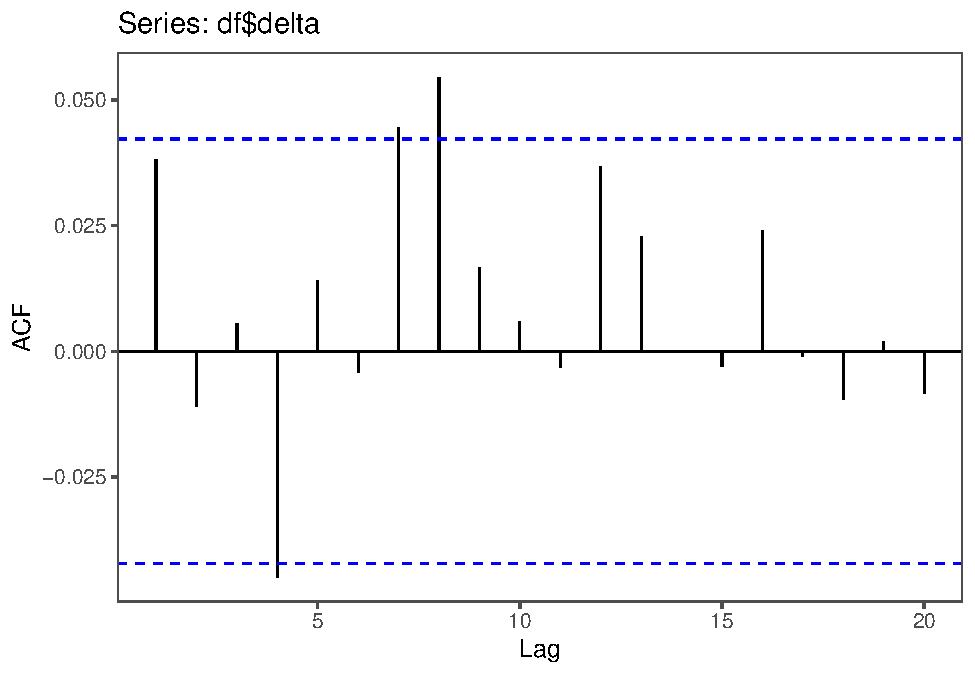
\includegraphics{Econo2_P1_files/figure-latex/plots-5} \end{center}

\begin{Shaded}
\begin{Highlighting}[]
\NormalTok{faclt}
\end{Highlighting}
\end{Shaded}

\begin{center}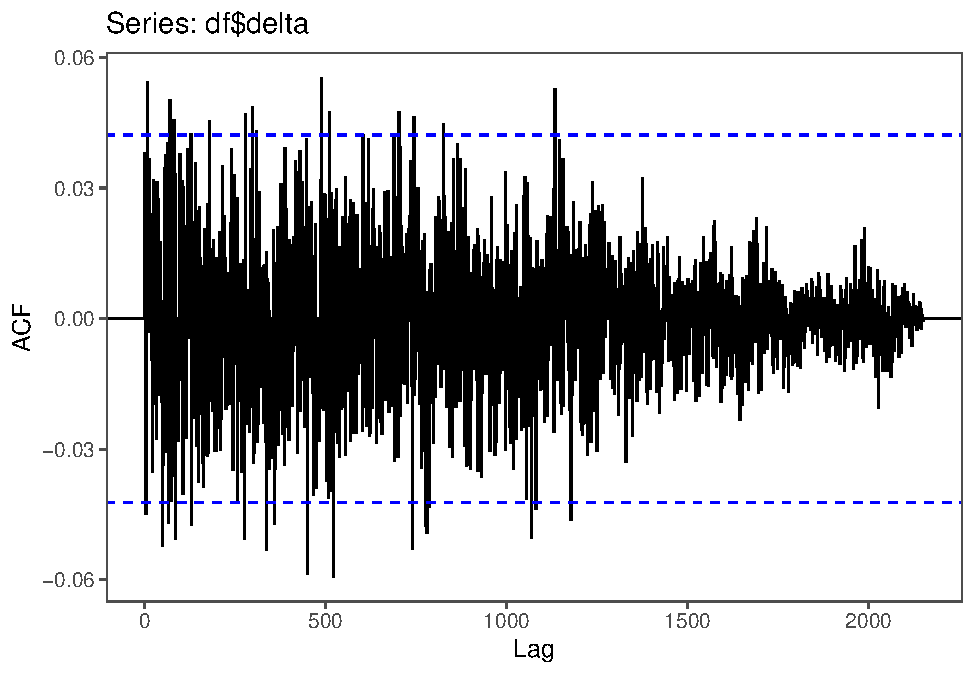
\includegraphics{Econo2_P1_files/figure-latex/plots-6} \end{center}

\begin{Shaded}
\begin{Highlighting}[]
\NormalTok{facpst}
\end{Highlighting}
\end{Shaded}

\begin{center}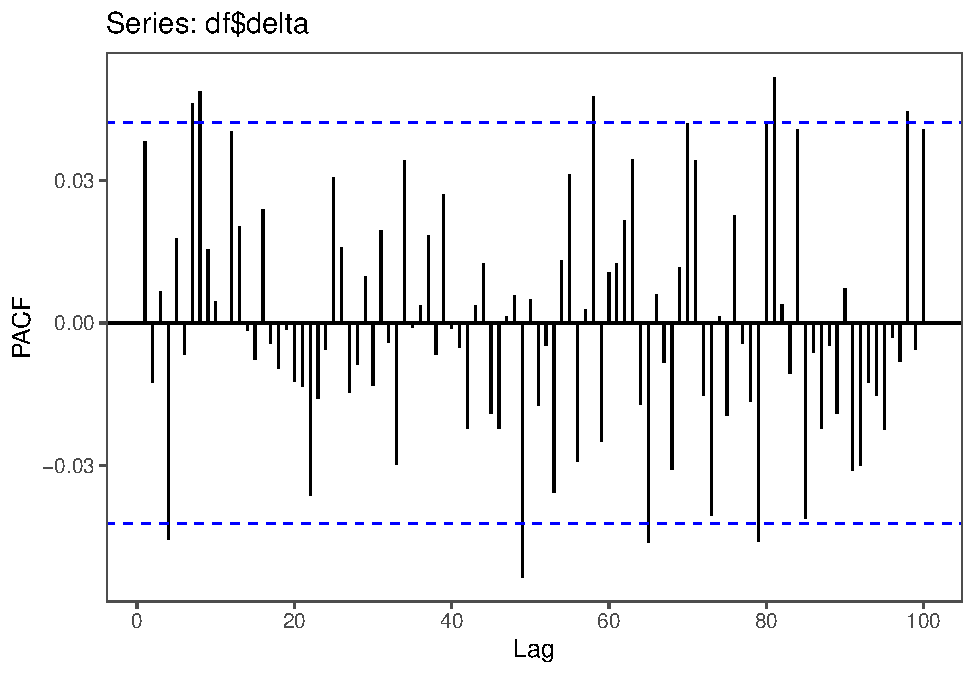
\includegraphics{Econo2_P1_files/figure-latex/plots-7} \end{center}

\begin{Shaded}
\begin{Highlighting}[]
\NormalTok{facplt}
\end{Highlighting}
\end{Shaded}

\begin{center}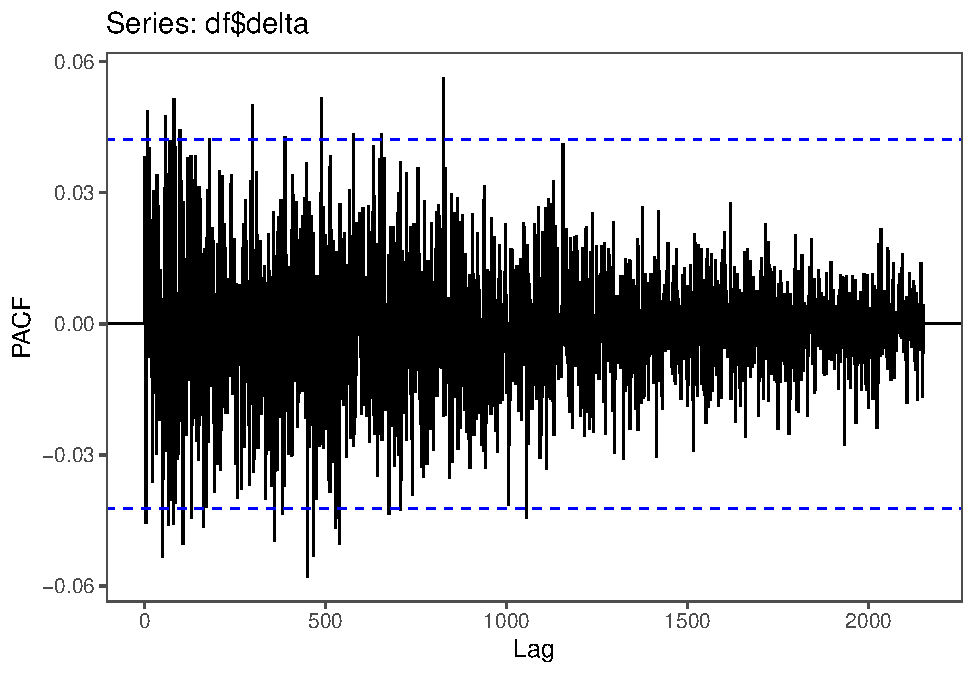
\includegraphics{Econo2_P1_files/figure-latex/plots-8} \end{center}

\begin{Shaded}
\begin{Highlighting}[]
\NormalTok{facst2 <-}\StringTok{ }\KeywordTok{ggAcf}\NormalTok{((df}\OperatorTok{$}\NormalTok{delta)}\OperatorTok{^}\DecValTok{2}\NormalTok{, }\DataTypeTok{type =} \StringTok{"correlation"}\NormalTok{, }\DataTypeTok{lag.max =} \DecValTok{20}\NormalTok{, }
    \DataTypeTok{plot =}\NormalTok{ T) }\OperatorTok{+}\StringTok{ }\KeywordTok{theme_few}\NormalTok{()}
\NormalTok{facst2}
\end{Highlighting}
\end{Shaded}

\begin{center}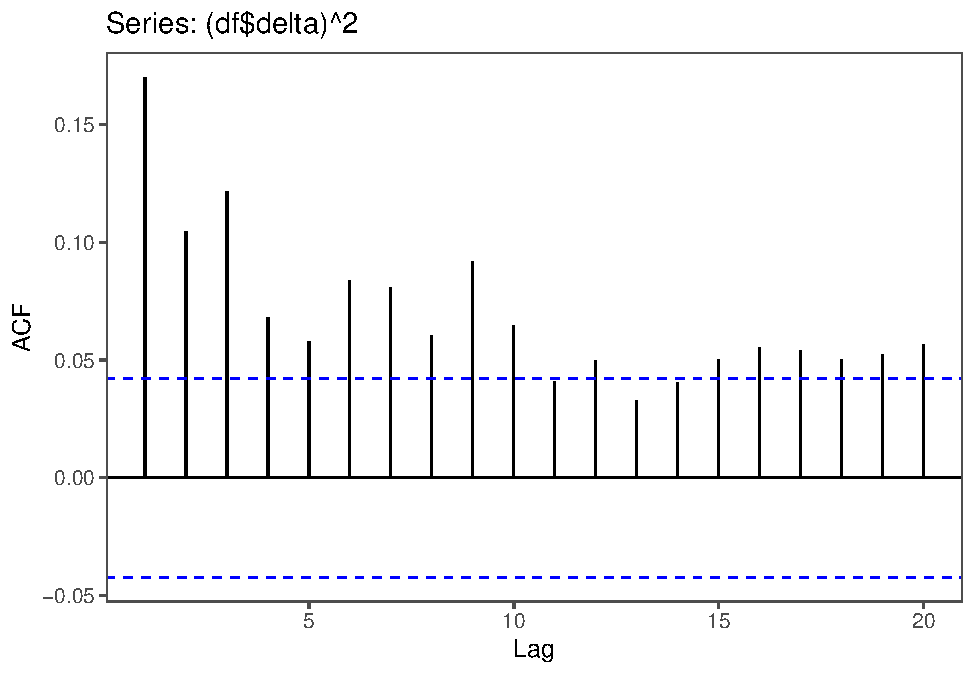
\includegraphics{Econo2_P1_files/figure-latex/plots-9} \end{center}

Let's now create our first ARMA models (equivalent to ARIMA with 2nd
argument = 0). We'll begin with the first hypothesis:
\(\mathbb{P}(+) = \mathbb{P}(-).\) Modelling this with an AR(1), we
have:

\[Sign_{t+1} = \alpha + \beta Sign_t + \varepsilon, \hspace{2em} \varepsilon \sim wn(0, \sigma^2)\]
In R, we'll use the package \emph{forecast} to construct this model:

\begin{Shaded}
\begin{Highlighting}[]
\NormalTok{AR1sign <-}\StringTok{ }\KeywordTok{Arima}\NormalTok{(df}\OperatorTok{$}\NormalTok{sign, }\DataTypeTok{order =} \KeywordTok{c}\NormalTok{(}\DecValTok{1}\NormalTok{, }\DecValTok{0}\NormalTok{, }\DecValTok{0}\NormalTok{))}
\KeywordTok{summary}\NormalTok{(AR1sign)}
\end{Highlighting}
\end{Shaded}

\begin{verbatim}
## Series: df$sign 
## ARIMA(1,0,0) with non-zero mean 
## 
## Coefficients:
##          ar1    mean
##       0.0278  0.5165
## s.e.  0.0215  0.0111
## 
## sigma^2 estimated as 0.2498:  log likelihood=-1560.63
## AIC=3127.26   AICc=3127.27   BIC=3144.28
## 
## Training set error measures:
##                        ME      RMSE       MAE  MPE MAPE     MASE          ACF1
## Training set 2.157119e-05 0.4995356 0.4990724 -Inf  Inf 1.027755 -0.0006313563
\end{verbatim}

\begin{Shaded}
\begin{Highlighting}[]
\KeywordTok{plot}\NormalTok{(AR1sign)}
\end{Highlighting}
\end{Shaded}

\begin{center}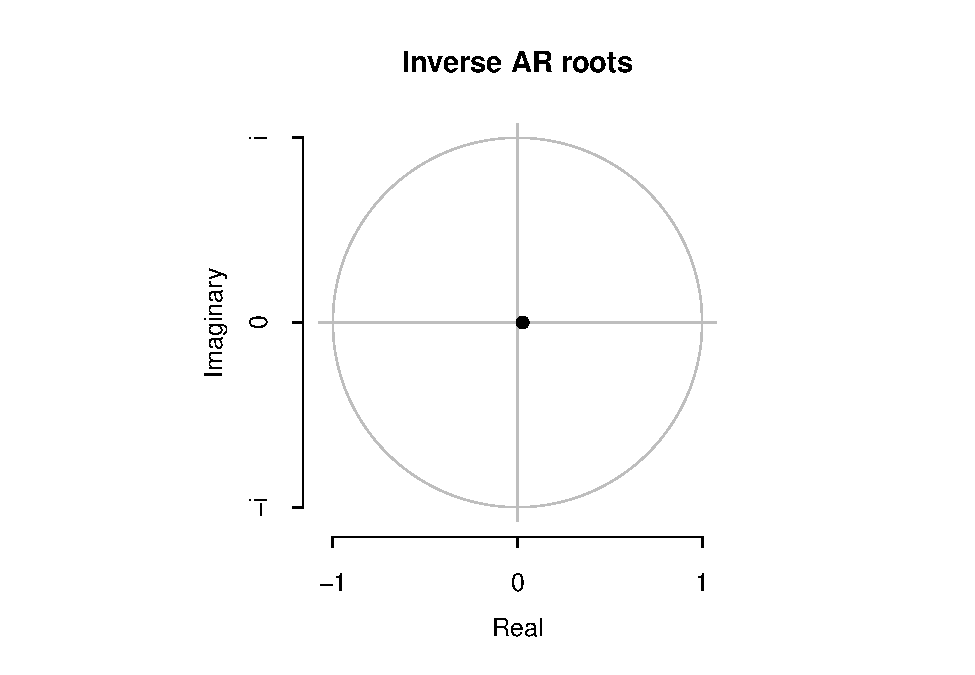
\includegraphics{Econo2_P1_files/figure-latex/AR(1)-1} \end{center}

\begin{Shaded}
\begin{Highlighting}[]
\KeywordTok{tsdisplay}\NormalTok{(AR1sign}\OperatorTok{$}\NormalTok{residuals)}
\end{Highlighting}
\end{Shaded}

\begin{center}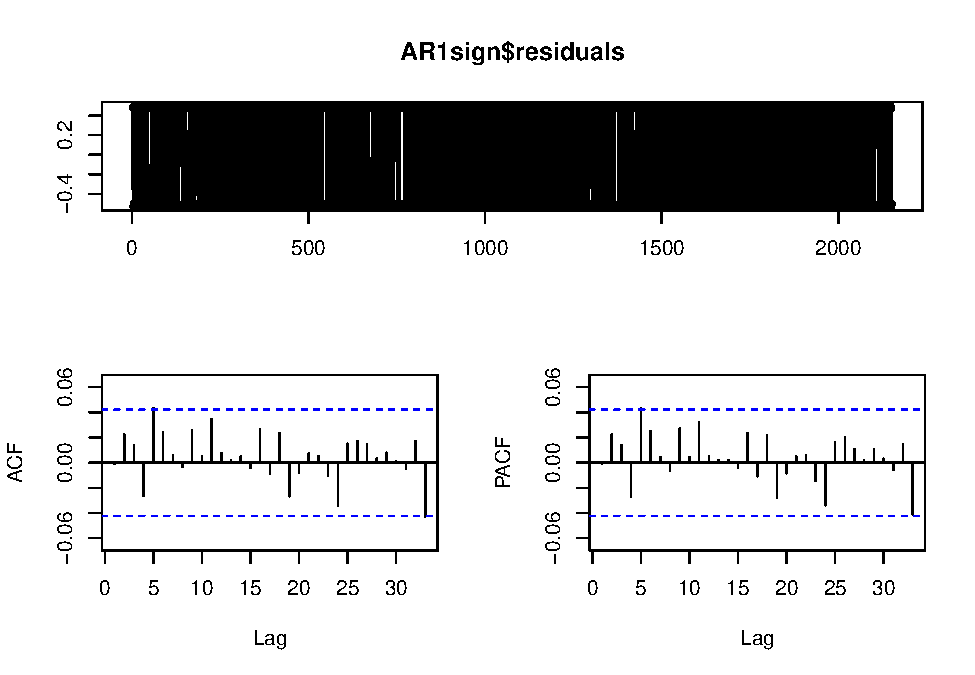
\includegraphics{Econo2_P1_files/figure-latex/AR(1)-2} \end{center}

With the results of the summary, we can now apply a hypothesis test for
our first
question.\footnote{Testing $\beta$ is equivalent to testing $\gamma$.}

\[ H_0: \beta = 0\] \[H_1: \beta \neq 0\]

\(\dfrac{\hat{ar_1} - ar_1}{s.e.(ar_1)}\):

\begin{Shaded}
\begin{Highlighting}[]
\NormalTok{AR1sign}\OperatorTok{$}\NormalTok{coef[}\DecValTok{1}\NormalTok{]}\OperatorTok{/}\KeywordTok{sqrt}\NormalTok{(AR1sign}\OperatorTok{$}\NormalTok{var.coef[}\DecValTok{1}\NormalTok{, }\DecValTok{1}\NormalTok{])}
\end{Highlighting}
\end{Shaded}

\begin{verbatim}
##      ar1 
## 1.287942
\end{verbatim}

The second hypothesis in the problem refers to the delta of the
variation: \[\mathbb{E}(\Delta | + ) \neq \mathbb{E}(\Delta | - ).\]

\[\Delta_{t+1} = \alpha + \beta Sign_t + \varepsilon, \hspace{2em} \varepsilon \sim wn(0, \sigma^2).\]

\begin{Shaded}
\begin{Highlighting}[]
\NormalTok{lmsignt <-}\StringTok{ }\KeywordTok{lm}\NormalTok{(delta }\OperatorTok{~}\StringTok{ }\KeywordTok{lag}\NormalTok{(df}\OperatorTok{$}\NormalTok{sign, }\DataTypeTok{k =} \DecValTok{1}\NormalTok{), }\DataTypeTok{data =}\NormalTok{ df)}
\KeywordTok{summary}\NormalTok{(lmsignt)}
\end{Highlighting}
\end{Shaded}

\begin{verbatim}
## 
## Call:
## lm(formula = delta ~ lag(df$sign, k = 1), data = df)
## 
## Residuals:
##     Min      1Q  Median      3Q     Max 
## -6.3285 -0.4706 -0.0060  0.4655  7.9442 
## 
## Coefficients:
##                     Estimate Std. Error t value Pr(>|t|)
## (Intercept)          0.01293    0.02811   0.460    0.646
## lag(df$sign, k = 1)  0.05802    0.03911   1.484    0.138
## 
## Residual standard error: 0.9066 on 2150 degrees of freedom
##   (1 observation deleted due to missingness)
## Multiple R-squared:  0.001023,   Adjusted R-squared:  0.000558 
## F-statistic: 2.201 on 1 and 2150 DF,  p-value: 0.1381
\end{verbatim}

\begin{Shaded}
\begin{Highlighting}[]
\KeywordTok{ggplot}\NormalTok{(df, }\KeywordTok{aes}\NormalTok{(}\DataTypeTok{x =} \KeywordTok{lag}\NormalTok{(df}\OperatorTok{$}\NormalTok{sign, }\DataTypeTok{k =} \DecValTok{1}\NormalTok{), }\DataTypeTok{y =}\NormalTok{ delta)) }\OperatorTok{+}\StringTok{ }\KeywordTok{geom_smooth}\NormalTok{(}\DataTypeTok{method =} \StringTok{"lm"}\NormalTok{)}
\end{Highlighting}
\end{Shaded}

\begin{verbatim}
## Warning: Use of `df$sign` is discouraged. Use `sign` instead.
\end{verbatim}

\begin{verbatim}
## `geom_smooth()` using formula 'y ~ x'
\end{verbatim}

\begin{verbatim}
## Warning: Removed 1 rows containing non-finite values (stat_smooth).
\end{verbatim}

\begin{center}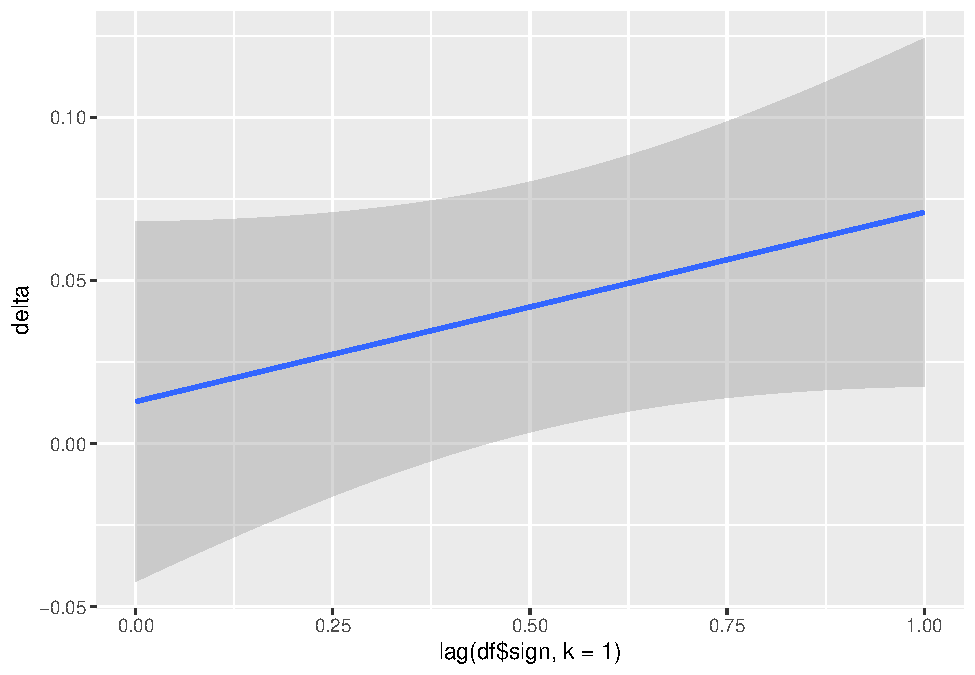
\includegraphics{Econo2_P1_files/figure-latex/lm signt-1} \end{center}

\[\Delta_{t+1} = \alpha + \beta_1 \Delta_t + \beta_2Sign_t + \varepsilon, \hspace{2em} \varepsilon \sim wn(0, \sigma^2)\]

\begin{Shaded}
\begin{Highlighting}[]
\NormalTok{AR1delta <-}\StringTok{ }\KeywordTok{Arima}\NormalTok{(df}\OperatorTok{$}\NormalTok{delta, }\DataTypeTok{order =} \KeywordTok{c}\NormalTok{(}\DecValTok{1}\NormalTok{, }\DecValTok{0}\NormalTok{, }\DecValTok{0}\NormalTok{), }\DataTypeTok{xreg =} \KeywordTok{lag}\NormalTok{(df}\OperatorTok{$}\NormalTok{sign, }
    \DataTypeTok{k =} \DecValTok{1}\NormalTok{))}
\KeywordTok{summary}\NormalTok{(AR1delta)}
\end{Highlighting}
\end{Shaded}

\begin{verbatim}
## Series: df$delta 
## Regression with ARIMA(1,0,0) errors 
## 
## Coefficients:
##          ar1  intercept    xreg
##       0.0321     0.0343  0.0166
## s.e.  0.0306     0.0351  0.0556
## 
## sigma^2 estimated as 0.8219:  log likelihood=-2840.96
## AIC=5689.93   AICc=5689.94   BIC=5712.62
## 
## Training set error measures:
##                        ME      RMSE      MAE MPE MAPE      MASE         ACF1
## Training set 1.147232e-05 0.9059341 0.643417 NaN  Inf 0.7252668 0.0003998294
\end{verbatim}

\begin{Shaded}
\begin{Highlighting}[]
\NormalTok{AR1delta}\OperatorTok{$}\NormalTok{coef[}\DecValTok{1}\NormalTok{]}\OperatorTok{/}\KeywordTok{sqrt}\NormalTok{(AR1delta}\OperatorTok{$}\NormalTok{var.coef[}\DecValTok{1}\NormalTok{, }\DecValTok{1}\NormalTok{])}
\end{Highlighting}
\end{Shaded}

\begin{verbatim}
##     ar1 
## 1.04747
\end{verbatim}

\begin{Shaded}
\begin{Highlighting}[]
\KeywordTok{plot}\NormalTok{(AR1delta)}
\end{Highlighting}
\end{Shaded}

\begin{center}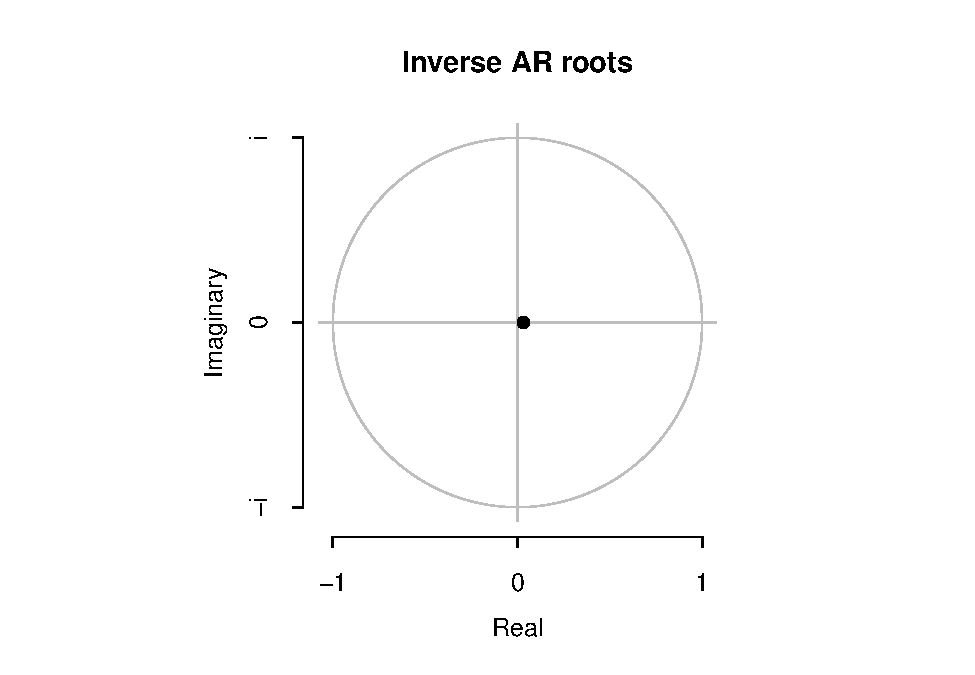
\includegraphics{Econo2_P1_files/figure-latex/delta 1-1} \end{center}

\begin{Shaded}
\begin{Highlighting}[]
\KeywordTok{tsdisplay}\NormalTok{(AR1delta}\OperatorTok{$}\NormalTok{residuals)}
\end{Highlighting}
\end{Shaded}

\begin{center}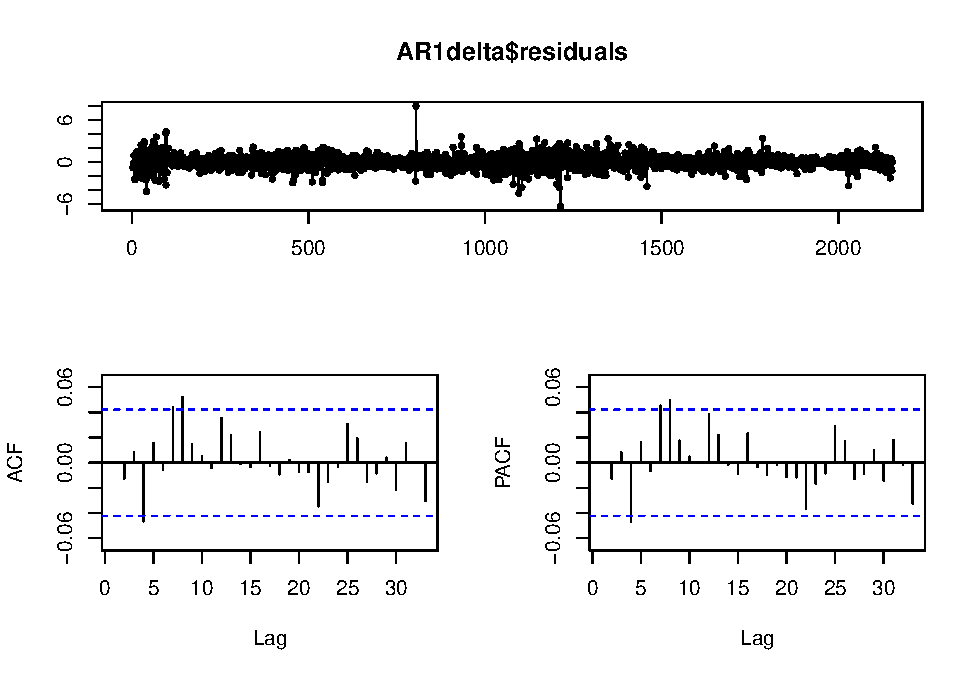
\includegraphics{Econo2_P1_files/figure-latex/delta 1-2} \end{center}

The last hypothesis in the problem refers to the variance:
\[\mathbb{E}(\Delta_{t+1}^2 | \Delta_t).\]

\[\Delta^2_{t+1} = \alpha + \beta \Delta^2_t + \varepsilon, \hspace{2em} \varepsilon \sim wn(0, \sigma^2)\]

\begin{Shaded}
\begin{Highlighting}[]
\NormalTok{AR1var <-}\StringTok{ }\KeywordTok{Arima}\NormalTok{((df}\OperatorTok{$}\NormalTok{delta)}\OperatorTok{^}\DecValTok{2}\NormalTok{, }\DataTypeTok{order =} \KeywordTok{c}\NormalTok{(}\DecValTok{1}\NormalTok{, }\DecValTok{0}\NormalTok{, }\DecValTok{0}\NormalTok{))}
\KeywordTok{summary}\NormalTok{(AR1var)}
\end{Highlighting}
\end{Shaded}

\begin{verbatim}
## Series: (df$delta)^2 
## ARIMA(1,0,0) with non-zero mean 
## 
## Coefficients:
##          ar1    mean
##       0.1701  0.8238
## s.e.  0.0212  0.0582
## 
## sigma^2 estimated as 5.026:  log likelihood=-4792.09
## AIC=9590.17   AICc=9590.18   BIC=9607.2
## 
## Training set error measures:
##                         ME     RMSE       MAE  MPE MAPE      MASE        ACF1
## Training set -6.299133e-05 2.240784 0.9197335 -Inf  Inf 0.8595655 -0.01320252
\end{verbatim}

\begin{Shaded}
\begin{Highlighting}[]
\NormalTok{AR1var}\OperatorTok{$}\NormalTok{coef[}\DecValTok{1}\NormalTok{]}\OperatorTok{/}\KeywordTok{sqrt}\NormalTok{(AR1var}\OperatorTok{$}\NormalTok{var.coef[}\DecValTok{1}\NormalTok{, }\DecValTok{1}\NormalTok{])}
\end{Highlighting}
\end{Shaded}

\begin{verbatim}
##      ar1 
## 8.011092
\end{verbatim}

\begin{Shaded}
\begin{Highlighting}[]
\KeywordTok{plot}\NormalTok{(AR1var)}
\end{Highlighting}
\end{Shaded}

\begin{center}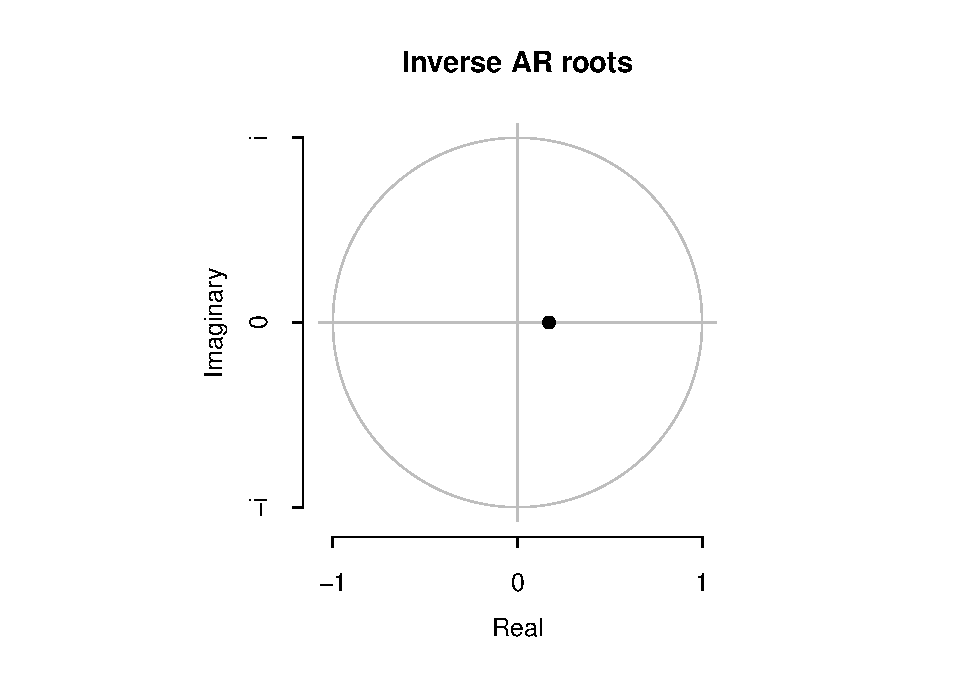
\includegraphics{Econo2_P1_files/figure-latex/var1-1} \end{center}

\begin{Shaded}
\begin{Highlighting}[]
\KeywordTok{tsdisplay}\NormalTok{(AR1var}\OperatorTok{$}\NormalTok{residuals)}
\end{Highlighting}
\end{Shaded}

\begin{center}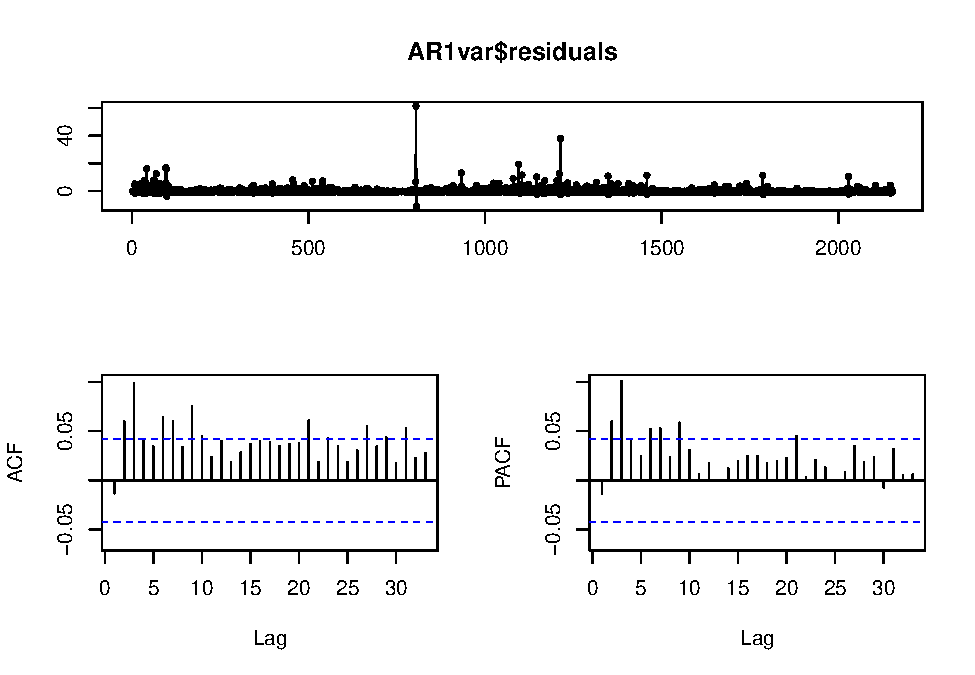
\includegraphics{Econo2_P1_files/figure-latex/var1-2} \end{center}

Now, let's run \emph{auto.arima}.

\begin{Shaded}
\begin{Highlighting}[]
\NormalTok{aadelta <-}\StringTok{ }\KeywordTok{auto.arima}\NormalTok{(df}\OperatorTok{$}\NormalTok{delta, }\DataTypeTok{stepwise =}\NormalTok{ F)}
\KeywordTok{summary}\NormalTok{(aadelta)}
\end{Highlighting}
\end{Shaded}

\begin{verbatim}
## Series: df$delta 
## ARIMA(1,0,1) with non-zero mean 
## 
## Coefficients:
##           ar1     ma1    mean
##       -0.7138  0.7506  0.0433
## s.e.   0.1486  0.1399  0.0199
## 
## sigma^2 estimated as 0.8208:  log likelihood=-2840.87
## AIC=5689.74   AICc=5689.76   BIC=5712.44
## 
## Training set error measures:
##                        ME      RMSE       MAE MPE MAPE    MASE        ACF1
## Training set 2.610156e-05 0.9053381 0.6434199 NaN  Inf 0.72527 0.003320553
\end{verbatim}

\begin{Shaded}
\begin{Highlighting}[]
\KeywordTok{plot}\NormalTok{(aadelta)}
\end{Highlighting}
\end{Shaded}

\begin{center}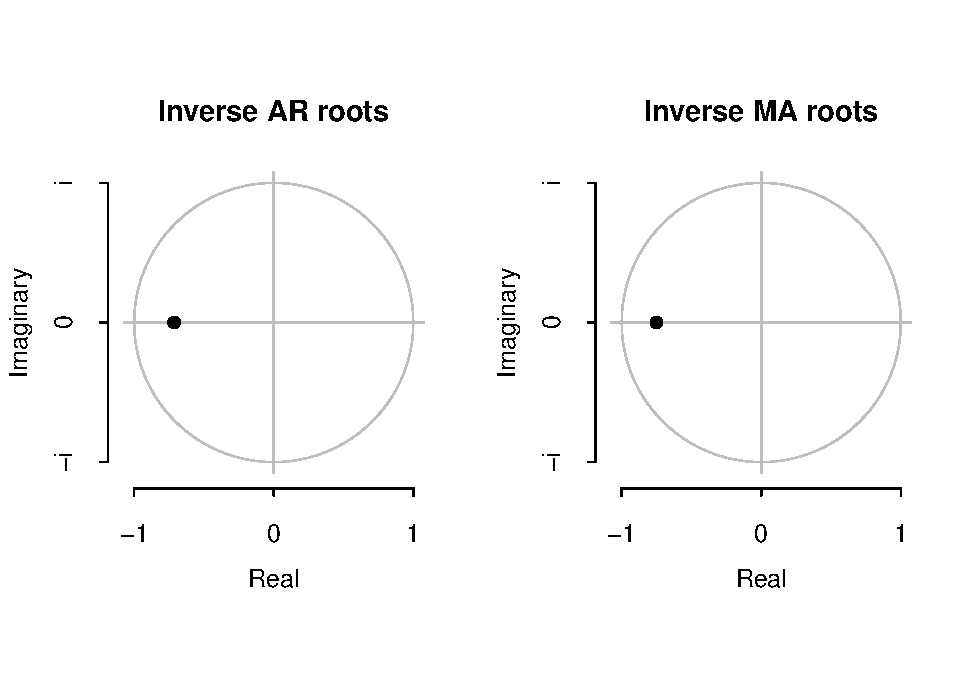
\includegraphics{Econo2_P1_files/figure-latex/auto arima-1} \end{center}

\begin{Shaded}
\begin{Highlighting}[]
\KeywordTok{tsdisplay}\NormalTok{(aadelta}\OperatorTok{$}\NormalTok{residuals)}
\end{Highlighting}
\end{Shaded}

\begin{center}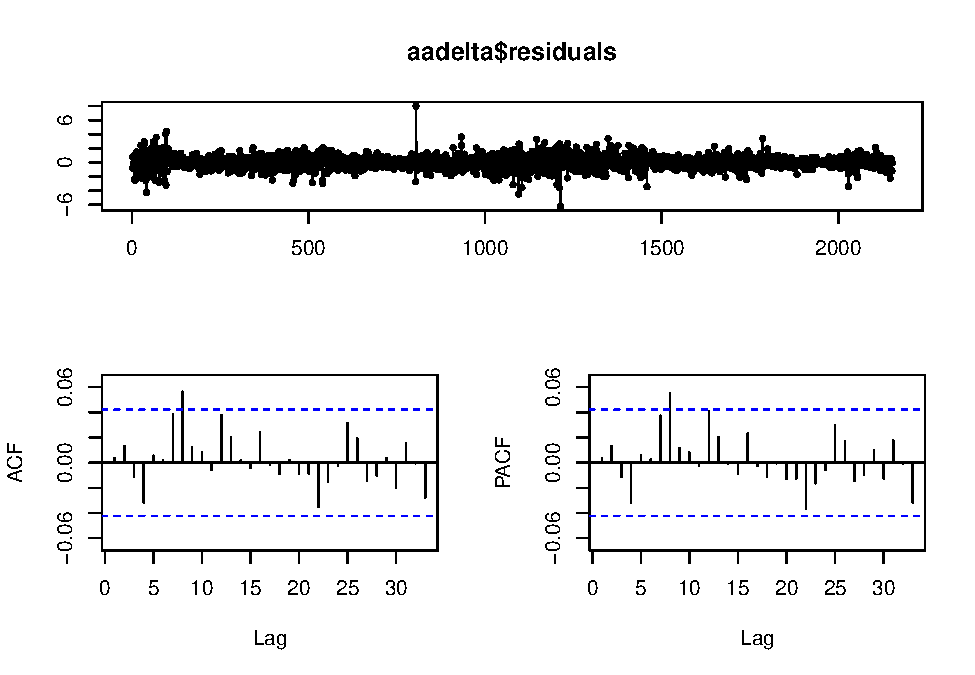
\includegraphics{Econo2_P1_files/figure-latex/auto arima-2} \end{center}

\begin{Shaded}
\begin{Highlighting}[]
\NormalTok{aasign <-}\StringTok{ }\KeywordTok{auto.arima}\NormalTok{(df}\OperatorTok{$}\NormalTok{sign, }\DataTypeTok{stepwise =}\NormalTok{ F)}
\KeywordTok{summary}\NormalTok{(aasign)}
\end{Highlighting}
\end{Shaded}

\begin{verbatim}
## Series: df$sign 
## ARIMA(0,0,0) with non-zero mean 
## 
## Coefficients:
##         mean
##       0.5165
## s.e.  0.0108
## 
## sigma^2 estimated as 0.2498:  log likelihood=-1561.46
## AIC=3126.91   AICc=3126.92   BIC=3138.26
## 
## Training set error measures:
##                         ME      RMSE       MAE  MPE MAPE     MASE       ACF1
## Training set -2.382602e-13 0.4997281 0.4994563 -Inf  Inf 1.028545 0.02773919
\end{verbatim}

\begin{Shaded}
\begin{Highlighting}[]
\KeywordTok{plot}\NormalTok{(aasign)}
\end{Highlighting}
\end{Shaded}

\begin{verbatim}
## Warning in plot.Arima(aasign): No roots to plot
\end{verbatim}

\begin{center}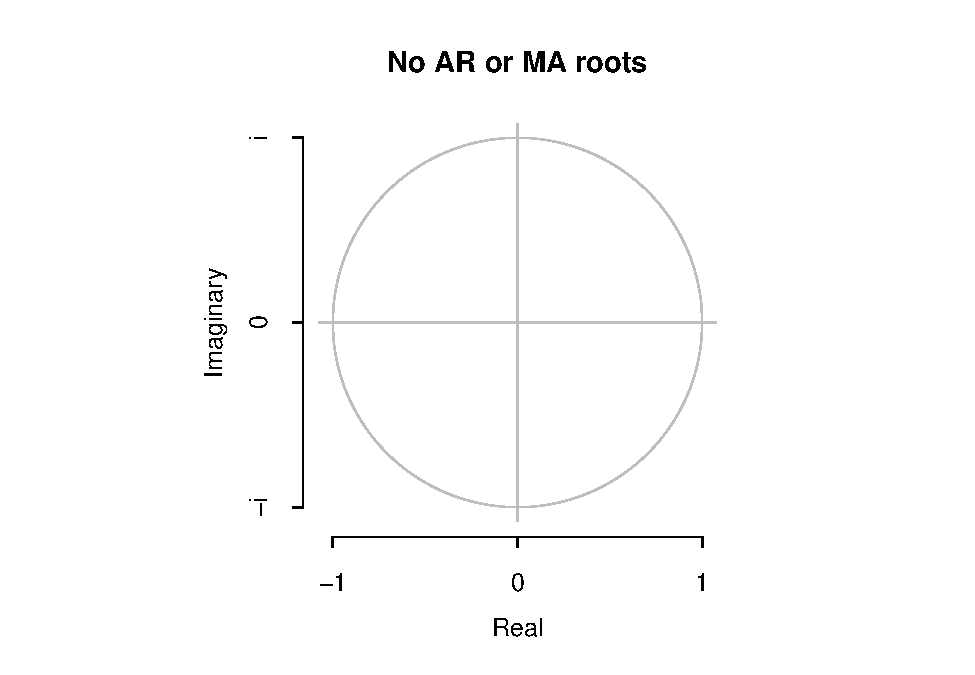
\includegraphics{Econo2_P1_files/figure-latex/auto arima-3} \end{center}

\begin{Shaded}
\begin{Highlighting}[]
\KeywordTok{tsdisplay}\NormalTok{(aasign}\OperatorTok{$}\NormalTok{residuals)}
\end{Highlighting}
\end{Shaded}

\begin{center}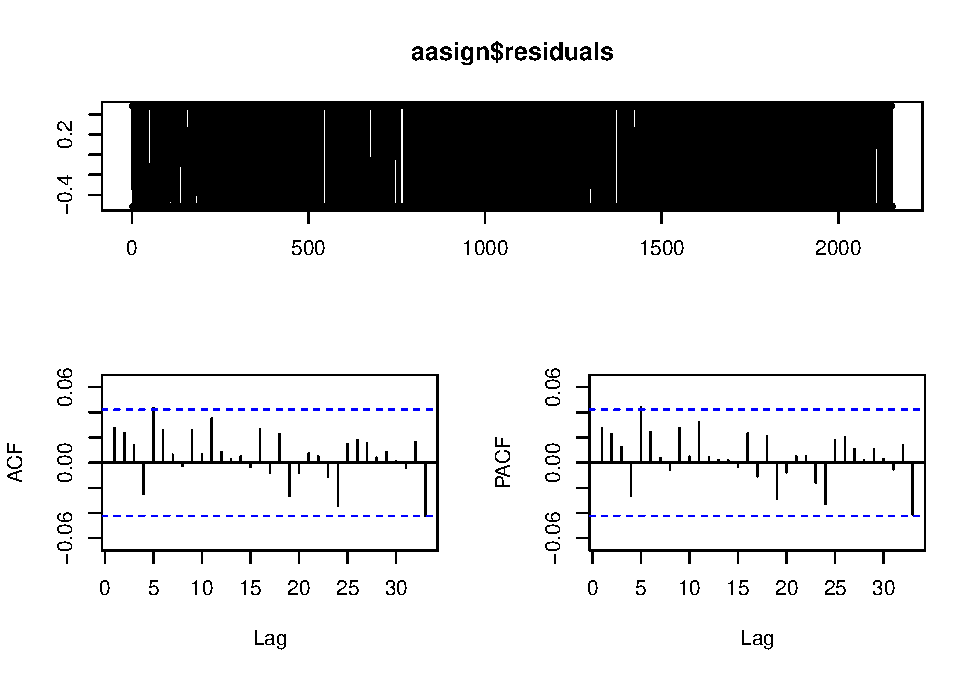
\includegraphics{Econo2_P1_files/figure-latex/auto arima-4} \end{center}

\begin{Shaded}
\begin{Highlighting}[]
\NormalTok{aavar <-}\StringTok{ }\KeywordTok{auto.arima}\NormalTok{((df}\OperatorTok{$}\NormalTok{delta)}\OperatorTok{^}\DecValTok{2}\NormalTok{, }\DataTypeTok{stepwise =}\NormalTok{ F)}
\KeywordTok{summary}\NormalTok{(aavar)}
\end{Highlighting}
\end{Shaded}

\begin{verbatim}
## Series: (df$delta)^2 
## ARIMA(0,1,4) 
## 
## Coefficients:
##           ma1      ma2     ma3      ma4
##       -0.8662  -0.0671  0.0228  -0.0641
## s.e.   0.0215   0.0284  0.0280   0.0214
## 
## sigma^2 estimated as 4.892:  log likelihood=-4761.22
## AIC=9532.45   AICc=9532.48   BIC=9560.82
## 
## Training set error measures:
##                       ME     RMSE       MAE  MPE MAPE      MASE         ACF1
## Training set -0.02170361 2.209213 0.8904046 -Inf  Inf 0.8321553 0.0001189823
\end{verbatim}

\begin{Shaded}
\begin{Highlighting}[]
\KeywordTok{plot}\NormalTok{(aavar)}
\end{Highlighting}
\end{Shaded}

\begin{center}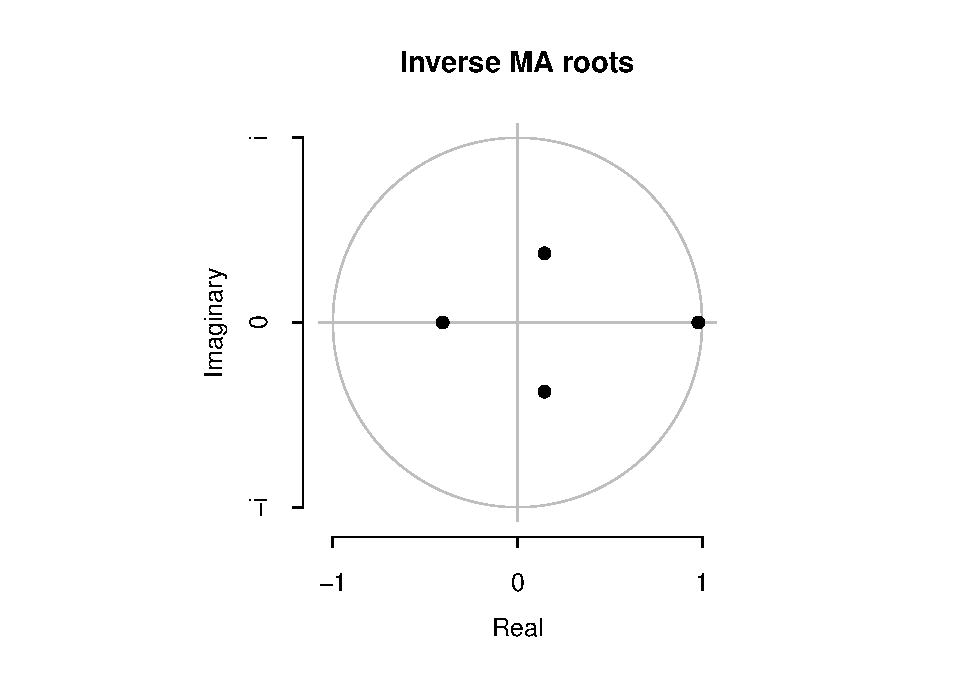
\includegraphics{Econo2_P1_files/figure-latex/auto arima-5} \end{center}

\begin{Shaded}
\begin{Highlighting}[]
\KeywordTok{tsdisplay}\NormalTok{(aasign}\OperatorTok{$}\NormalTok{residuals)}
\end{Highlighting}
\end{Shaded}

\begin{center}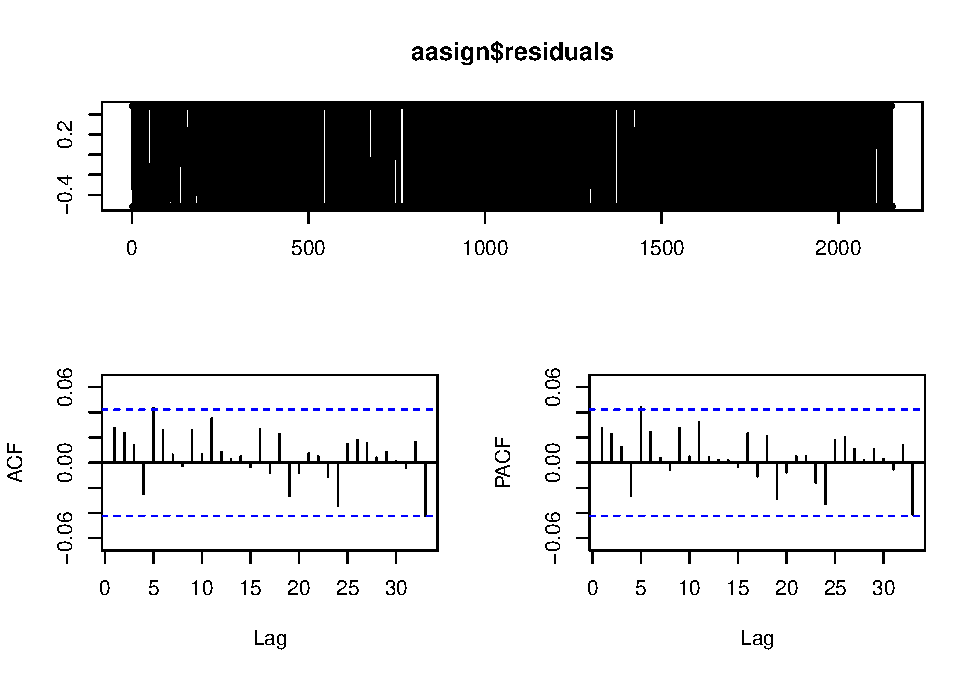
\includegraphics{Econo2_P1_files/figure-latex/auto arima-6} \end{center}

\begin{Shaded}
\begin{Highlighting}[]
\NormalTok{aardelta <-}\StringTok{ }\KeywordTok{auto.arima}\NormalTok{(df}\OperatorTok{$}\NormalTok{delta, }\DataTypeTok{max.q =} \DecValTok{0}\NormalTok{, }\DataTypeTok{stepwise =}\NormalTok{ F)}
\KeywordTok{summary}\NormalTok{(aardelta)}
\end{Highlighting}
\end{Shaded}

\begin{verbatim}
## Series: df$delta 
## ARIMA(1,0,0) with non-zero mean 
## 
## Coefficients:
##          ar1    mean
##       0.0382  0.0433
## s.e.  0.0215  0.0203
## 
## sigma^2 estimated as 0.8215:  log likelihood=-2842.26
## AIC=5690.52   AICc=5690.53   BIC=5707.54
## 
## Training set error measures:
##                         ME      RMSE       MAE MPE MAPE      MASE         ACF1
## Training set -1.464203e-05 0.9059233 0.6434299 NaN  Inf 0.7252813 0.0004805619
\end{verbatim}

\begin{Shaded}
\begin{Highlighting}[]
\KeywordTok{plot}\NormalTok{(aardelta)}
\end{Highlighting}
\end{Shaded}

\begin{center}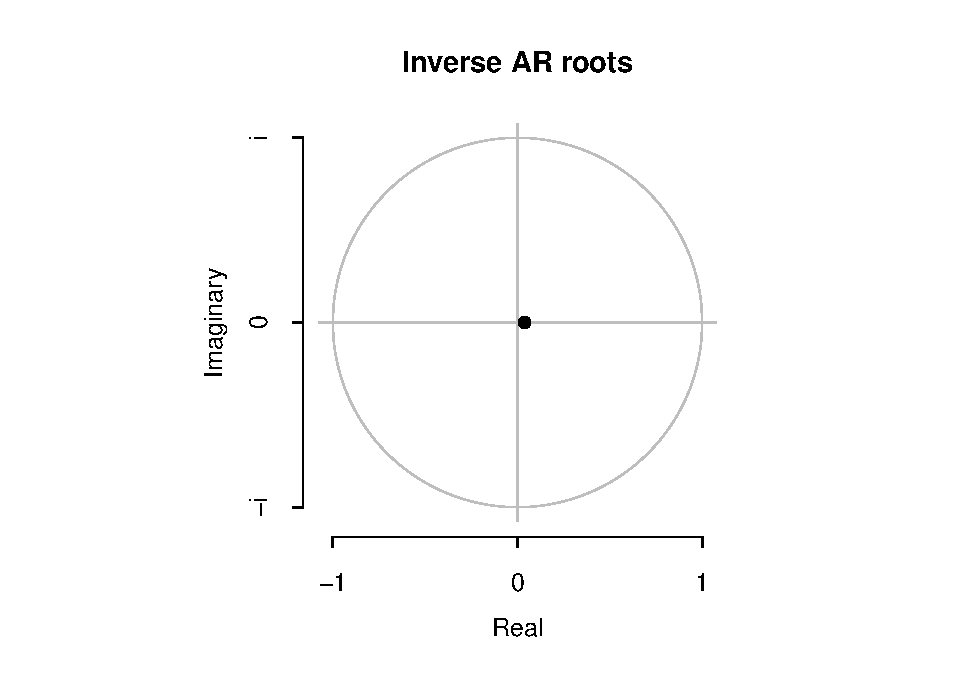
\includegraphics{Econo2_P1_files/figure-latex/auto arima-7} \end{center}

\begin{Shaded}
\begin{Highlighting}[]
\KeywordTok{tsdisplay}\NormalTok{(aardelta}\OperatorTok{$}\NormalTok{residuals)}
\end{Highlighting}
\end{Shaded}

\begin{center}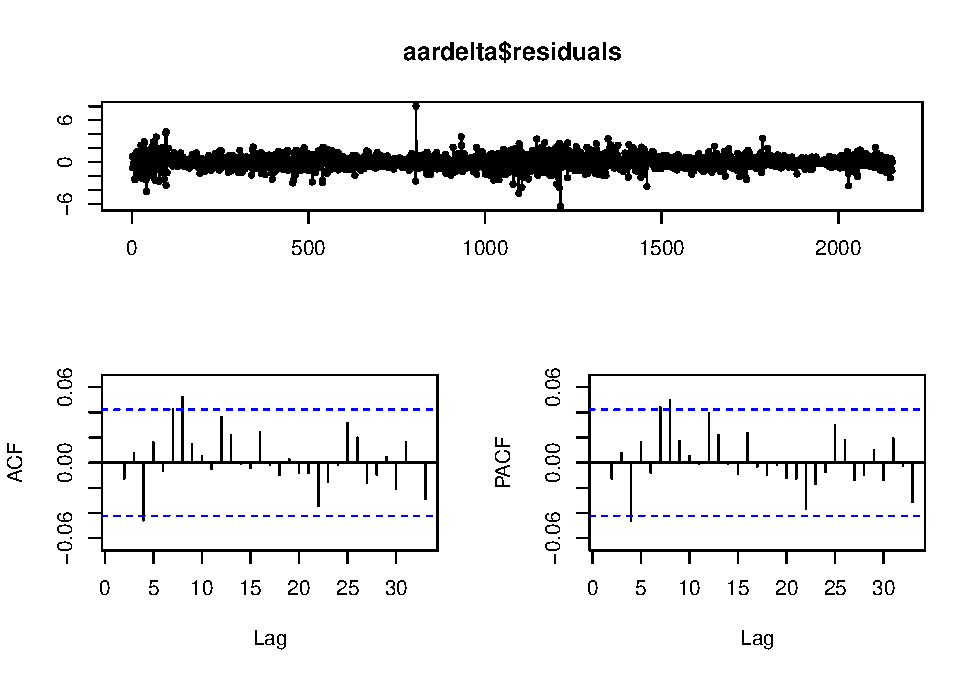
\includegraphics{Econo2_P1_files/figure-latex/auto arima-8} \end{center}

\begin{Shaded}
\begin{Highlighting}[]
\NormalTok{aarsign <-}\StringTok{ }\KeywordTok{auto.arima}\NormalTok{(df}\OperatorTok{$}\NormalTok{sign, }\DataTypeTok{max.q =} \DecValTok{0}\NormalTok{, }\DataTypeTok{stepwise =}\NormalTok{ F)}
\KeywordTok{summary}\NormalTok{(aarsign)}
\end{Highlighting}
\end{Shaded}

\begin{verbatim}
## Series: df$sign 
## ARIMA(0,0,0) with non-zero mean 
## 
## Coefficients:
##         mean
##       0.5165
## s.e.  0.0108
## 
## sigma^2 estimated as 0.2498:  log likelihood=-1561.46
## AIC=3126.91   AICc=3126.92   BIC=3138.26
## 
## Training set error measures:
##                         ME      RMSE       MAE  MPE MAPE     MASE       ACF1
## Training set -2.382602e-13 0.4997281 0.4994563 -Inf  Inf 1.028545 0.02773919
\end{verbatim}

\begin{Shaded}
\begin{Highlighting}[]
\KeywordTok{plot}\NormalTok{(aarsign)}
\end{Highlighting}
\end{Shaded}

\begin{verbatim}
## Warning in plot.Arima(aarsign): No roots to plot
\end{verbatim}

\begin{center}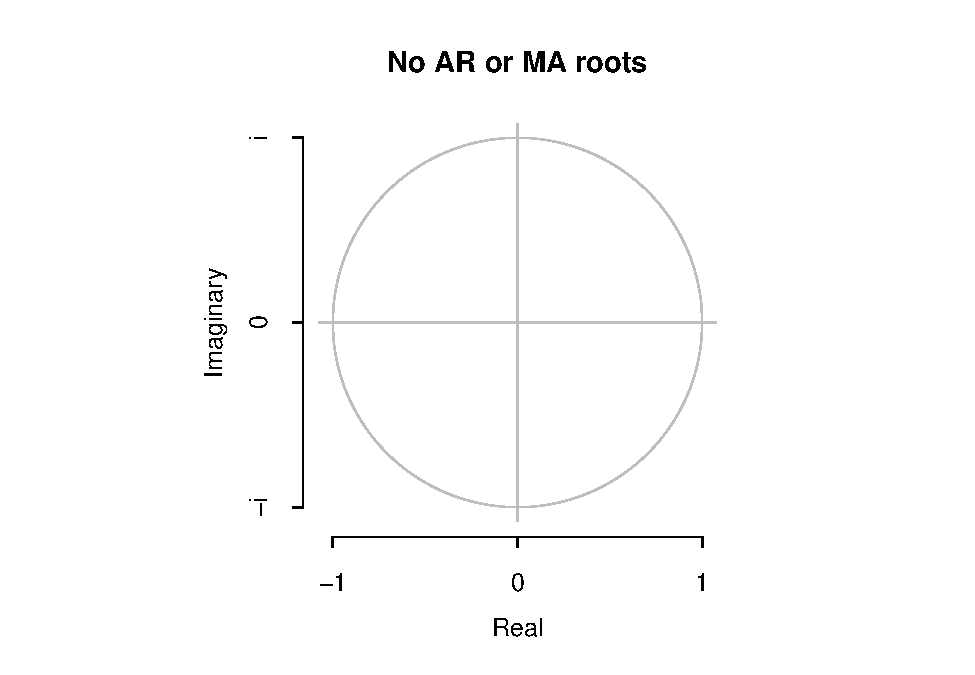
\includegraphics{Econo2_P1_files/figure-latex/auto arima-9} \end{center}

\begin{Shaded}
\begin{Highlighting}[]
\KeywordTok{tsdisplay}\NormalTok{(aarsign}\OperatorTok{$}\NormalTok{residuals)}
\end{Highlighting}
\end{Shaded}

\begin{center}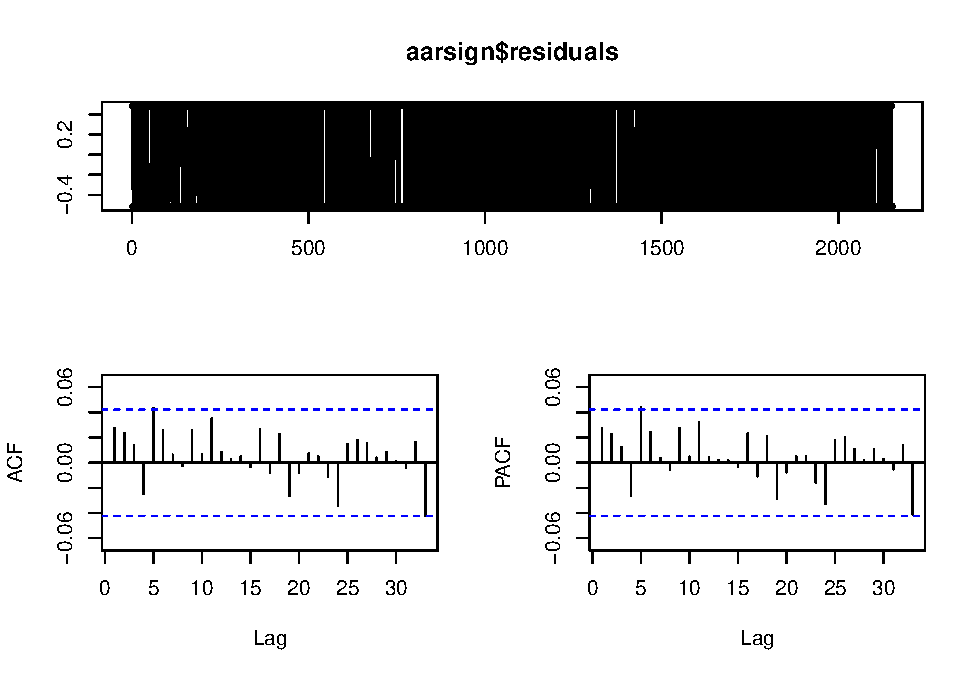
\includegraphics{Econo2_P1_files/figure-latex/auto arima-10} \end{center}

\begin{Shaded}
\begin{Highlighting}[]
\NormalTok{aarvar <-}\StringTok{ }\KeywordTok{auto.arima}\NormalTok{((df}\OperatorTok{$}\NormalTok{delta)}\OperatorTok{^}\DecValTok{2}\NormalTok{, }\DataTypeTok{max.q =} \DecValTok{0}\NormalTok{, }\DataTypeTok{stepwise =}\NormalTok{ F)}
\KeywordTok{summary}\NormalTok{(aarvar)}
\end{Highlighting}
\end{Shaded}

\begin{verbatim}
## Series: (df$delta)^2 
## ARIMA(5,1,0) 
## 
## Coefficients:
##           ar1      ar2      ar3      ar4      ar5
##       -0.7420  -0.5845  -0.4042  -0.2873  -0.1687
## s.e.   0.0213   0.0259   0.0274   0.0258   0.0212
## 
## sigma^2 estimated as 5.465:  log likelihood=-4878.95
## AIC=9769.89   AICc=9769.93   BIC=9803.94
## 
## Training set error measures:
##                         ME     RMSE       MAE  MPE MAPE      MASE       ACF1
## Training set -3.234587e-05 2.334504 0.9170278 -Inf  Inf 0.8570369 -0.0239684
\end{verbatim}

\begin{Shaded}
\begin{Highlighting}[]
\KeywordTok{plot}\NormalTok{(aarvar)}
\end{Highlighting}
\end{Shaded}

\begin{center}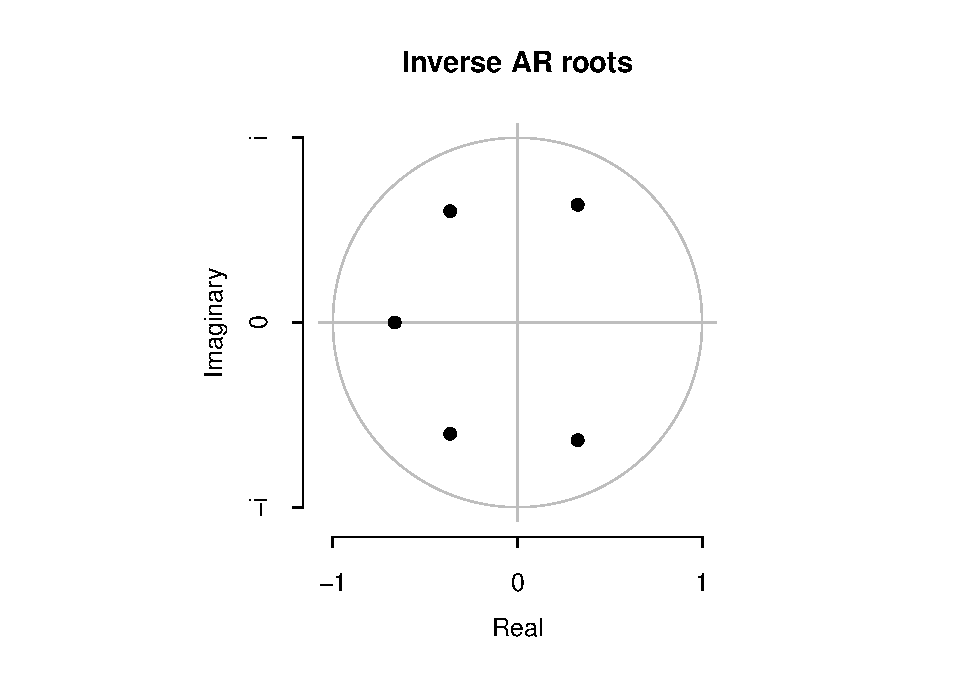
\includegraphics{Econo2_P1_files/figure-latex/auto arima-11} \end{center}

\begin{Shaded}
\begin{Highlighting}[]
\KeywordTok{tsdisplay}\NormalTok{(aarvar}\OperatorTok{$}\NormalTok{residuals)}
\end{Highlighting}
\end{Shaded}

\begin{center}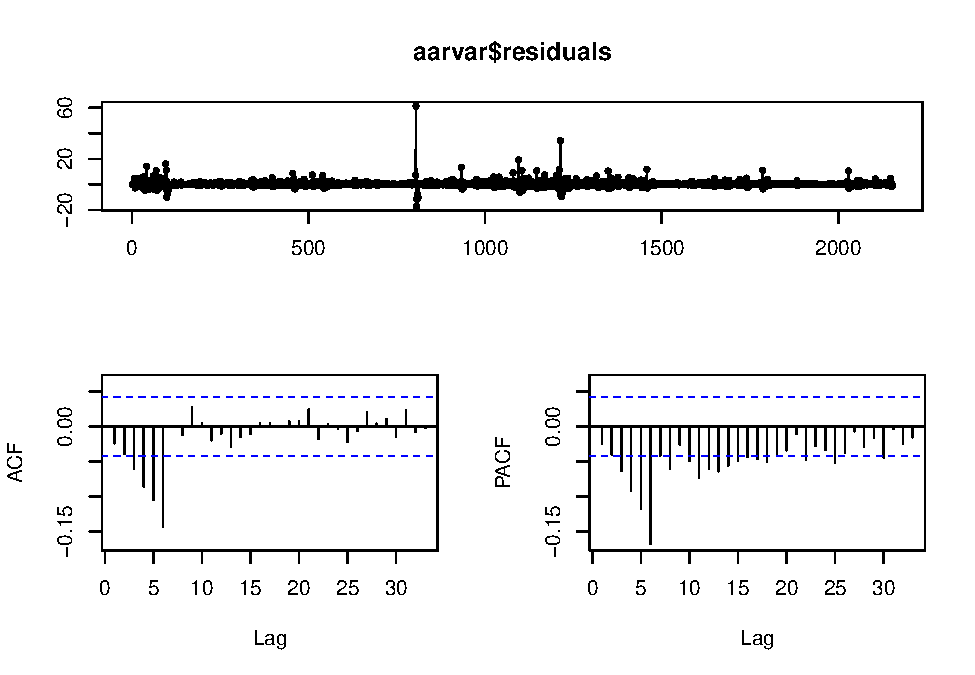
\includegraphics{Econo2_P1_files/figure-latex/auto arima-12} \end{center}

\[ \Delta_{t+1} = c + \beta \Delta_t + \varepsilon\]

\begin{Shaded}
\begin{Highlighting}[]
\NormalTok{AR1_}\DecValTok{2}\NormalTok{ <-}\StringTok{ }\KeywordTok{Arima}\NormalTok{(df}\OperatorTok{$}\NormalTok{delta, }\DataTypeTok{order =} \KeywordTok{c}\NormalTok{(}\DecValTok{1}\NormalTok{, }\DecValTok{0}\NormalTok{, }\DecValTok{0}\NormalTok{))}

\KeywordTok{summary}\NormalTok{(AR1_}\DecValTok{2}\NormalTok{)}
\end{Highlighting}
\end{Shaded}

\begin{verbatim}
## Series: df$delta 
## ARIMA(1,0,0) with non-zero mean 
## 
## Coefficients:
##          ar1    mean
##       0.0382  0.0433
## s.e.  0.0215  0.0203
## 
## sigma^2 estimated as 0.8215:  log likelihood=-2842.26
## AIC=5690.52   AICc=5690.53   BIC=5707.54
## 
## Training set error measures:
##                         ME      RMSE       MAE MPE MAPE      MASE         ACF1
## Training set -1.464203e-05 0.9059233 0.6434299 NaN  Inf 0.7252813 0.0004805619
\end{verbatim}

\begin{Shaded}
\begin{Highlighting}[]
\KeywordTok{confint}\NormalTok{(AR1_}\DecValTok{2}\NormalTok{, }\DataTypeTok{level =} \FloatTok{0.95}\NormalTok{)}
\end{Highlighting}
\end{Shaded}

\begin{verbatim}
##                  2.5 %     97.5 %
## ar1       -0.003988796 0.08042284
## intercept  0.003511958 0.08308440
\end{verbatim}

\end{document}
